\documentclass[conference]{IEEEtran}

\usepackage[utf8]{inputenc}
\usepackage{amsmath, amsfonts}
\usepackage{graphicx}
\usepackage[table]{xcolor}
\usepackage{multirow}
\usepackage{colortbl}
\usepackage{hyperref}
\usepackage{caption}
\usepackage{float}
\definecolor{MyLightPurple}{RGB}{204, 204, 255}
\usepackage{pgfplots}
\pgfplotsset{compat=1.18}
\usepackage{pgfplotstable}

\title{Título del Artículo IEEE}

\author{
    \IEEEauthorblockN{Autor Uno}
    \IEEEauthorblockA{
        Facultad de Ingeniería\\
        Universidad Ejemplo\\
        Ciudad, País\\
        \texttt{autor1@ejemplo.com}
    }
    \and
    \IEEEauthorblockN{Autor Dos}
    \IEEEauthorblockA{
        Departamento de Ciencias\\
        Otra Universidad\\
        Ciudad, País\\
        \texttt{autor2@ejemplo.com}
    }
}

\begin{document}
    \maketitle
        \begin{abstract}
            Tarea del curso de Metodología de la Investigación
        \end{abstract}
    
        \begin{IEEEkeywords}
            IEEE, LaTeX, artículo, plantilla, dos columnas.
        \end{IEEEkeywords}
    
        \section{Introducción}
        Adicionar a este template los siguientes elementos:
            \begin{itemize}
                \item Tabla multicolumna y multifila
                \item Figura con caption descriptivo
                \item Por lo menos 2 ítems en la bibliografía (archivo bibliografia.bib) y colocar la referencia con el comando cite en el texto.
            \end{itemize}
        Todos los elementos tienen que aparecer en un lugar determinado por el alumno en el código.\\
        \indent Este es un ejemplo mínimo de documento con formato IEEE y dos columnas. 
        La clase \verb|IEEEtran| se usa comúnmente para conferencias y publicaciones científicas.
    
        
        
        
        \section{Ecuaciones Matemáticas}
        
            \LaTeX{}  es una excelente herramienta para escribir ecuaciones
            matemáticas, como por ejemplo: \(x = a^2 + b^2 + c^2\). También expresiones más complejas:
                \begin{equation}
                    \gamma^2 + \theta^2 = \omega^2
                \end{equation}
            
            \noindent
            ``Las ecuaciones de Maxwell's'' fueron nombradas por 
            James Clark Maxwell y están descritas a continuación (para las ecuaciones usa el entorno \textbf{align} del paquete \verb|\usepackage{amsmath}| y \verb|\label{etiqueta}| para colocar una etiqueta en la ecuación):
            
            \setcounter{equation}{1}
            \begin{gather}
                \vec{\nabla} \cdot \vec{E} = \frac{\rho}{\varepsilon_0} \qquad \text{Gauss's Law} \label{eq:gauss1} \\
                \vec{\nabla} \cdot \vec{B} = 0 \qquad \text{Gauss's Law for Magnetism} \label{eq:gauss2}
            \end{gather}
    
            \noindent 
            Las Ecuaciones ~\ref{eq:gauss1} y \ref{eq:gauss2} son las mas importantes para el área 
            de Física (referenciado con el comando \verb|\ref{etiqueta}|
            
            \subsection{Ecuaciones con matrices (sin numeración)}
            
            La siguinte ecuación puede ser recreada usando los entornos
            pmatrix, vmatrix y matrix del entorno equation*, el símbolo * hace  que no se considere numeración para esa ecuación.
        
            \begin{equation*}
                \begin{pmatrix}
                a_{11} & a_{12} & \cdots & a_{1n}\\
                a_{21} & a_{22} & \cdots & a_{2n}\\
                \vdots & \vdots & \ddots & \vdots\\
                a_{n1} & a_{n2} & \cdots & a_{nn}
                \end{pmatrix}
                \begin{bmatrix}
                v_1\\ v_2\\ \vdots\\ v_n
                \end{bmatrix}
                =
                \begin{bmatrix}
                w_1\\ w_2\\ \vdots\\ w_n
                \end{bmatrix}.
            \end{equation*}
    
        
        \section{Tablas}
            Para reproducir la Tabla I, se deben emplear los siguientes comandos:
            \begin{itemize}
                \item \verb|\usepackage[table]{xcolor}|      y 
                        \verb|\usepackage{colorbtl}|: Permiten aplicar colores a las filas y columnas, mejorando la legibilidad.
                \item \verb|\columncolor{color}c|: Comando utilizado para colorear columnas específicas sin afectar la alineación, y se coloca dentro de las definiciones de columna del entorno tabular, es por ello  que se visualiza el comando \verb|c| después del columncolor\verb|{color}|
                \item \verb|\rowcolor{color}|: Se usa para colorear filas específicas (como el encabezado) con un color más destacado
            \end{itemize}
            
            \begin{table}[t]
                \centering
                % Configuración de estilo de la tabla
                \setlength{\tabcolsep}{3pt} % espacio entre columnas
                %\renewcommand{\arraystretch}{0.8} % altura de las filas
                % Definición de la tabla y sus colores
                \begin{tabular}{| >{\columncolor{MyLightPurple}} c | c | c | c |}
                    % Fila del encabezado con color de fondo
                    \hline
                    \rowcolor{gray!20}
                    \textbf{Tamaño entrenamiento} & \textbf{Clasificador A} & \textbf{Clasificador B} & \textbf{Clasificador C} \\
                    % Filas de datos
                    10 & 65 & 60 & \textbf{70} \\
                    30 & 72 & 68 & \textbf{75} \\
                    50 & 78 & 75 & \textbf{82} \\
                    70 & 85 & \textbf{88} & 87 \\
                    90 & 88 & \textbf{93} & 90 \\
                    \hline
                \end{tabular} 
                \captionsetup{      
                    labelsep=newline,         
                    justification=centering,    
                    singlelinecheck=false,   
                    font=scriptsize       
                }
                \caption{
                 ACCURACY (\%) PARA LOS CLASIFICADORES SEGÚN EL TAMAÑO DEL CONJUNTO DE ENTRENAMIENTO, EN NEGRITA EL MEJOR RESULTADO OBTENIDO.}
                \label{tab:resultados}
            \end{table}
    
        
        \section{Graficos}
            \begin{figure}[H]
                \centering
                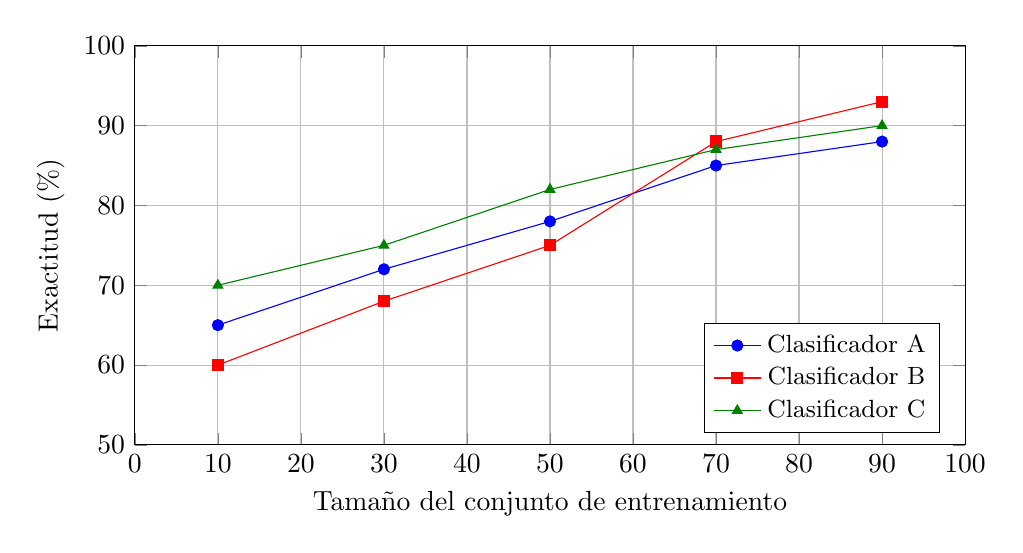
\begin{tikzpicture}
                    \begin{axis}[
                        width=\linewidth,
                        height=6.65cm,
                        grid=both,
                        xlabel={Tamaño del conjunto de entrenamiento},
                        ylabel={Exactitud (\%)},
                        xmin= 0, xmax = 100,
                        ymin=50, ymax=100,
                        ytick={50,60,70,80,90,100},
                        legend style={
                            at={(0.97,0.03)}, % Cerca de la esquina inferior derecha
                            anchor=south east, % Anclaje en la esquina sur-este de la caja de leyenda
                            legend columns=1,  % Que sea una columna vertical (como en la imagen)
                            fill=white,        
                            draw=black,      
                            font=\small    
                        },
                        cycle list={
                        {blue, mark=*,       every mark/.append style={fill=blue}},    
                        {red, mark=square*,  every mark/.append style={fill=red}},     
                        {green!50!black, mark=triangle*, every mark/.append style={fill=green!50!black}}
                        }
                    ]
                
                    \addplot coordinates {(10,65) (30,72) (50,78) (70,85) (90,88)};
                    \addlegendentry{Clasificador A}
                    
                    \addplot coordinates {(10,60) (30,68) (50,75) (70,88) (90,93)};
                    \addlegendentry{Clasificador B}
                    
                    \addplot coordinates {(10,70) (30,75) (50,82) (70,87) (90,90)};
                    \addlegendentry{Clasificador C} 
                        \end{axis}
                    \end{tikzpicture}
                    
                    \caption{\small Comparación de desempeño de clasificadores}
                    \label{fig:comparacion}
            \end{figure}
            
            
            Para reproducir el Gráfico de Líneas, mostrando en la Figura \textbf{??}, se aplican  las siguientes técnicas:
            \begin{itemize}
                \item \verb|\usepackage{pgfplots}|: Este paquete permite la creación de gráficos de alta calidad.
                \item \verb|\pgfplotsset{compat=1.18}|: Asegura la compatibilidad con la versión específica de PGFPlots, garantizando la estabilidad y funciones avanzadas.
                \item \verb|\begin{axis}| y \verb|\end{axis|: Se utiliza para definir el área del gráfico donde se ubicarán los ejes, las leyendas y los datos.
                \item \verb|xtick=data| y  \verb|xticklabels={Precisión,|
                \verb| Recall, F1-Score}|: Define los puntos de las etiquetas del eje x y asigna etiquetas personalizadas para cada métrica.
                \item \verb|ymin=0.0, ymax=1.1|: Configura el rango de valores del eje \verb|y|, ajustando el gráfico a una escala de 0 a 1.1
                \item \verb|\addplot|:  Este comando agrega los datos del gráfico ´
                de líneas. Cada modelo (Regresión Logística, Bosques
                Aleatorios y Red Neuronal) se agrega con coordenadas
                específicas.
                \item \verb|legend style={at={(0.5,-0.2)},| 
                \verb|anchor=north, legend columns=3}|: Configura la leyenda del gráfico, colocándola debajo del gráfico y distribuyéndola en tres columnas.
                \item \verb|grid=both|: Añade líneas de cuadrícula al gráfico para mejorar la lectura y la comparación visual entre las curvas.
                \item \verb|mark=square, mark=triangle*, mark=o|: Se utilizan para especificar diferentes marcadores en cada línea,
                mejorando la distinción visual entre los modelos. 
            \end{itemize}
        
        \section{Referencias}
        
        %\bibliographystyle{IEEEtran}
        \bibliography{bibliografia}
\end{document}

    



